\documentclass[aspectratio=169,dvipsnames,svgnames,10pt]{beamer}

\usepackage[T1]{fontenc}
\usepackage[utf8]{inputenc}
\usepackage[french, english]{babel}
\selectlanguage{english}

\usepackage{graphicx}

% Math
\usepackage{amsmath}
% \usepackage{amsfonts}
\usepackage{amssymb}
\usepackage{amsthm}
% \usepackage{mathrsfs}
\usepackage{mathtools}
\usepackage{textcomp}
% \usepackage{textgreek}

% Specialized packages
% \usepackage{syntax} % Grammar definitions
\usepackage{subcaption}
\usepackage{verbatim}
\usepackage{listings} % Code
\usepackage{xspace} % Useful for macros
\usepackage{natbib}% Good citations and bibliography
\usepackage{mathpartir} % Syntax trees
\usepackage{colortbl}
\usepackage{multicol}%multicolumn lists
\usepackage{minted}
\setminted{encoding=utf-8}
\usepackage{pifont}

% \usepackage{mathptmx}
% \usepackage[scaled=0.9]{helvet}
\usepackage{beramono}

\usepackage{natbib}
\bibliographystyle{abbrvnat}

\usepackage{appendixnumberbeamer}

\usetheme{metropolis}
\beamertemplatenavigationsymbolsempty
\setbeamercovered{transparent=20}
\metroset{
  sectionpage=none,
  numbering=fraction,
  progressbar=foot,
}

\makeatletter
\newenvironment{btHighlight}[1][]
{\begingroup\tikzset{bt@Highlight@par/.style={#1}}\begin{lrbox}{\@tempboxa}}
{\end{lrbox}\bt@HL@box[bt@Highlight@par]{\@tempboxa}\endgroup}

\newcommand\btHL[1][]{%
  \begin{btHighlight}[#1]\bgroup\aftergroup\bt@HL@endenv%
}
\def\bt@HL@endenv{%
  \end{btHighlight}%   
  \egroup
}
\newcommand{\bt@HL@box}[2][]{%
  \tikz[#1]{%
    \pgfpathrectangle{\pgfpoint{1pt}{0pt}}{\pgfpoint{\wd #2}{\ht #2}}%
    \pgfusepath{use as bounding box}%
    \node[anchor=base west, fill=orange!30,outer sep=0pt,inner xsep=1pt, inner ysep=0pt, rounded corners=3pt, minimum height=\ht\strutbox+1pt,#1]{\raisebox{1pt}{\strut}\strut\usebox{#2}};
  }%
}
\makeatother
\lstset{
  basicstyle=\ttfamily,
  columns=fullflexible,
  keepspaces=true,
  moredelim=**[is][\btHL]{`}{`},
  extendedchars=true,
  literate={µ}{{\textmu}}1
}

\newcommand\Y{{\color{Green}{\ding{52}}}\xspace}
\newcommand\N{{\color{Red}{\ding{56}}}\xspace}
\newcommand\M{{\color{Orange}{\textasciitilde}}\xspace} % "Meh"

\def\HUGE{\fontsize{35pt}{15pt}\selectfont}

\title{Isomorphisms are back!}
\subtitle{Smart indexing for search by types in libraries}
\author{
  Clément \textsc{Allain}
  \and
  \underline{Gabriel \textsc{Radanne}}
  \and
  Laure \textsc{Gonnord} \\
}

\date{}


\begin{document}

\lstMakeShortInline[keepspaces,basicstyle=\small\ttfamily]@

\begin{frame}
  \titlepage
\end{frame}

\begin{frame}[fragile]
  \frametitle{Problem}

  Every programmer has encountered this problem once:

  \begin{quotation}
    I'm looking for a function that does X, where to find it?
  \end{quotation}

  Often there is an ``intuitive'' approach: I want a function
  on time, I look in the {\color{orange}\tt Time} module.
  This does not always work (auxiliary modules \dots).

  $\Rightarrow$ We can search functions using a very familiar abstraction: their types!
  
\end{frame}

\begin{frame}[fragile]
  \frametitle{Our tool: Dowsing!}
\begin{itemize}
\item Finds types ``up to'' order of arguments, instantiation, \dots
\item Knows about packages/libraries
\item Scales to modern ecosystems (for instance, opam)
\end{itemize}
  \vfill
  \begin{columns}
    \column{0.6\textwidth}
    \footnotesize
\begin{verbatim}
$ search "'a list * 'a -> bool"
...
List.mem : 'a -> 'a list -> bool
...

$ search "'a list -> ('a * 'b -> 'b) -> 'b -> 'b"
...
List.fold_left :
  ('a -> 'b -> 'a) -> 'a -> 'b list -> 'a
List.fold_right :
  ('a -> 'b -> 'b) -> 'a list -> 'b -> 'b
...
\end{verbatim}
    \column{0.4\textwidth}
    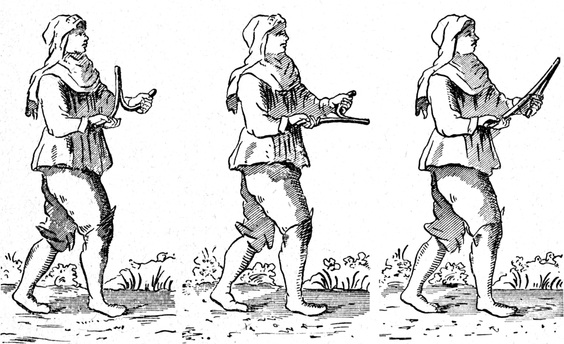
\includegraphics{sourcier}
  \end{columns}
\pause
How does it all work ?
\end{frame}

\begin{frame}
  \frametitle{Existing approaches}

  {\large Search by type modulo isomorphism}:
  \begin{itemize}
  \item Sound and complete \Y
  \item Computationally intensive \N
  \end{itemize}

  \vfill

  {\large Hoogle} (\url{https://hoogle.haskell.org/}):
  \begin{itemize}
  \item Neither sound nor complete (more like ``text search in types'') \N
  \item Scales well \Y
  \end{itemize}
\end{frame}

\begin{frame}
  \frametitle{Search by type modulo isomorphism}

  Given a type $\tau$, finds all functions in the libraries with types \\
  which are equivalent/match/unify to $\tau$ up to some set\\
  of ``simplifications''.

  We consider the following simplifications (i.e., isomorphisms):
\begin{align}
    a \times b &\equiv_T
    b \times a
    \label{prod_comm}
    \tag{$\times$-comm}
  \\
    a \times (b \times c) &\equiv_T
    (a \times b) \times c
    \label{prod_assoc}
    \tag{$\times$-assoc}
  \\
    \texttt{unit} \times a &\equiv_T
    a
    \label{prod_unit}
    \tag{$\times$-$\texttt{unit}$}
  \\
    (a \times b) \rightarrow c &\equiv_T
    a \rightarrow (b \rightarrow c)
    \label{curry}
    \tag{curry}
\end{align}
  
  {\color{red} Problem}: Unification/Matching modulo isomorphism is \emph{expensive}.
\end{frame}

\begin{frame}
  \frametitle{Smart indexing}

  Some remarks:
  \begin{itemize}
  \item When searching, many types do not match
  \item Even when failing, unification is expensive
  \item Performance of unification highly depends on the types (more than $*1000$ variance)
  \end{itemize}
  \pause
  \vfill
  
  Battle plan:
  \begin{enumerate}
  \item Experimentally measure to identify types taking lots of time
  \item Introduces ``shortcuts'', to skip unification for these expensive types
  \item Pre-process the database of types to compute shortcuts in advance
  \item Rinse and repeat
  \end{enumerate}
  
\end{frame}

\begin{frame}[fragile]
  \frametitle{Example of metric: The head}
Exemples:
\begin{itemize}
  \item $head(unit \rightarrow \textcolor{orange}{\alpha}) = \bold{var}$
  \item $head(int \rightarrow int \rightarrow \textcolor{orange}{list} (\alpha)) = \bold{cons}_{list}$
\end{itemize}
\bigskip
\begin{lstlisting}
$ stats "int -> int -> int" --measure head
measure        total time (ms)    avg. time (µs)    # unif.
------------------------------------------------------------
variable       506.137            `311.086`            `1627`
constructor    62.705             2.45229            25570
tuple          11.2598            2.73429            4118
other          0.815153           3.09944            263
\end{lstlisting}
Observations:
\begin{itemize}
  \item 95\% without variables at the head
  \item Case with variable head are pathological
\end{itemize}

\end{frame}


\begin{frame}[fragile]
  \frametitle{Example of shortcut: Head matching}

  If two types have incompatible heads, they can never unify:
\begin{itemize}
  \item 
    $\dots \rightarrow \textcolor{orange}{int} \not\equiv_T$ 
    $\dots \rightarrow \textcolor{orange}{float}$
  \item
    $\dots \rightarrow \textcolor{orange}{list} (\alpha) \not\equiv_T$ 
    $\dots \rightarrow int \,\textcolor{orange}{\times}\, int$
  \item
    $\dots \rightarrow \textcolor{orange}{int} \stackrel{?}{\equiv}_T$ 
    $\dots \rightarrow \textcolor{orange}{\alpha}$
  \end{itemize}

  We precompute the heads for all types in the database and store them compactly
\end{frame}

\begin{frame}[fragile]
  \frametitle{Example of shortcut: Head matching -- benchmarking}
  Searching in a local install of opam:\\
  $\sim 250$ packages, $31578$ functions
\begin{table}[h]
  \small
  \centering
  \begin{tabular}{|*{3}{c|}}
    \hline
      Type &
      Nb unif. w shortcut &
      Gain
    \\
    \hline
      $int \rightarrow int \rightarrow int$ &
      2714 & \textcolor{teal}{91.4\%}
    \\
      $int \rightarrow int \rightarrow int \rightarrow int$ &
      2714 & \textcolor{teal}{91.4\%}
    \\
      $int \rightarrow (int \rightarrow int) \rightarrow list (\alpha)$ &
      2945 & 90.7\%
    \\
      $int \rightarrow float \rightarrow bool \rightarrow \bold{unit}$ &
      5745 & \textcolor{violet}{81.8\%}
    \\
      $\alpha \rightarrow int \rightarrow \bold{unit}$ &
      5745 & \textcolor{violet}{81.8\%}
    \\
      $int \rightarrow int \rightarrow \alpha$ &
      31578 & \textcolor{orange}{0\%}
    \\
    \hline
  \end{tabular}
\end{table}

\begin{itemize}
\item We correctly avoid many unifications
\item We need to work more for polymorphic queries
\end{itemize}
\end{frame}

\begin{frame}
  \frametitle{More shortcuts and combinations}

  We introduced more shortcuts (and plan to investigate more):
  \begin{itemize}
  \item Number of variables at the tail
  \item Relative positions of variables
  \end{itemize}

  \vfill

  \begin{columns}
    \column{0.6\textwidth}
    {\Large How to combine them?}\\
    We use a trie-like structure of ``features''.\\
    Given a query (here, a constructor $f$), we select all sub-tries
    with potentially valid types.
    \column{0.4\textwidth}
    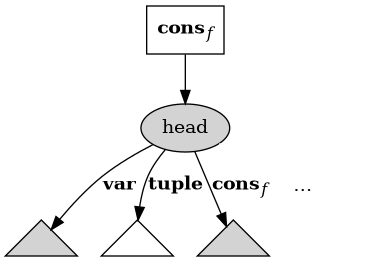
\includegraphics[width=\textwidth]{crit1_3}
  \end{columns}

\end{frame}


\begin{frame}[fragile]
  \frametitle{Final benchmark}

  Benchmark on database containing containers, batteries and base:\\
  $\sim 10000$ functions
\begin{table}[h]
  \centering
  \begin{tabular}{|*{4}{c|}}
    \hline
      Type &
      Nb unif. w shortcuts &
      Time (ms)
    \\
    \hline
      $int \rightarrow int \rightarrow int$ &
      50 & 0.368ms 
    \\
      $int \rightarrow int \rightarrow int \rightarrow int$ &
      45 & 0.649ms 
    \\
      $int \rightarrow (int \rightarrow int) \rightarrow list (\alpha)$ &
      67 & 0.415ms 
    \\
      $int \rightarrow float \rightarrow bool \rightarrow \bold{unit}$ &
      62 & 1.26ms 
    \\
      $\alpha \rightarrow int \rightarrow \bold{unit}$ &
      62 & 0.592ms 
    \\
      $int \rightarrow int \rightarrow \alpha$ &
      29 & 0.393ms 
    \\
      $list(\alpha) \rightarrow \_ \rightarrow \alpha$ &
      642 & 391ms 
    \\
    \hline
  \end{tabular}

\end{table}
  $\Rightarrow$ Instant in practice for many queries. Still work to do on very
  polymorphic queries
\end{frame}


\begin{frame}
  \frametitle{Conclusion}

  We presented \emph{Dowsing}, a new approach to search in libraries by types:
  \begin{itemize}
  \item Sound and complete
  \item Scales well to medium ecosystem (and beyond?)
  \item Good methodological approach to improve it further
  \end{itemize}
  
  Our technique is formalized and implemented: \url{https://github.com/Drup/dowsing/}
\end{frame}

\begin{frame}
  \frametitle{Ongoing work}

  \begin{columns}
    \raggedleft
    \begin{column}{0.4\textwidth}
      
    Lot's of work to do to make this practical!

    \vspace{1em}
    Indexing:
    \begin{itemize}
    \item Add more feature
    \item Invent new kinds of shortcuts
    \end{itemize}
    \vspace{1em}

    Type system:\\
    \begin{itemize}
    \item Add more OCaml features
    \end{itemize}

    \vspace{1em}
    
    Software development:
    \begin{itemize}
    \item Plug this into opam CI
    \item Develop a web-based frontend
    \end{itemize}
    \end{column}
        
    \column{0.28\textwidth}
    
\includegraphics[width=\textwidth]{weneedyou.jpg}
    \column{0.3\textwidth}
    
  \end{columns}
  
\end{frame}

\end{document}

%%% Local Variables:
%%% mode: latex
%%% TeX-master: t
%%% TeX-command-extra-options: "-shell-escape"
%%% End:
